\documentclass[conference]{IEEEtran}
\IEEEoverridecommandlockouts
% The preceding line is only needed to identify funding in the first footnote. If that is unneeded, please comment it out.
\usepackage{hyperref}
\usepackage{comment}
\usepackage{cite}
\usepackage{amsmath,amssymb,amsfonts}
\usepackage{algorithmic}
\usepackage{graphicx}
\usepackage{textcomp}
\usepackage{xcolor}
\usepackage{cleveref}
\def\BibTeX{{\rm B\kern-.05em{\sc i\kern-.025em b}\kern-.08em
    T\kern-.1667em\lower.7ex\hbox{E}\kern-.125emX}}
\begin{document}

\title{Remote Monitoring and  Control of Mobile Robots in Real-Time Using Multimodal Digital Twins}

\author{\IEEEauthorblockN{Trung Kien La}
\IEEEauthorblockA{\textit{Dept. of Comp. Science \& Engineering} \\
\textit{Frankfurt University of Applied Sciences}\\
Frankfurt a.M., Germany \\
trung.la@stud.fra-uas.de}
\and
\IEEEauthorblockN{René Harmann}
\IEEEauthorblockA{\textit{Dept. of Comp. Science \& Engineering} \\
\textit{Frankfurt University of Applied Sciences}\\
Frankfurt a.M., Germany\\
rene.harmann@fb2.fra-uas.de}
\and
\IEEEauthorblockN{Eric Guiffo Kaigom}
\IEEEauthorblockA{\textit{Dept. of Comp. Science \& Engineering} \\
\textit{Frankfurt University of Applied Sciences}\\
Frankfurt a.M., Germany \\
kaigom@fb2.fra-uas.de}

}

\maketitle

\begin{abstract}
    Although digital twins have been playing a pivotal role in the management of the lifecycle of physical robotic systems of systems, they have hardly been employed to actively guide mobile robots in real-time. 
    In fact, 
    the guidance of such systems
    requires functionalities, including the perception of  environmental constraints and avoidance of collisions. A spatial
    information stream beyond the internal robot state measured using
    proprioceptive sensors is therefore needed. Exteroceptive sensors help
    meet this demand. Nevertheless, such sensors have received little
    attention thus far in the development of digital twins. On the
    other hand, various mobility objectives, such as
    reverse motions, might require the awareness of the historical
    internal state of the distant robot. For instance, the current
    energy budget is likely to constrain the  reachability of the
    initial robot location, even when spatially and kinematically
    feasible. We therefore develop a web-based framework to monitor and actively steer mobile robots while leveraging on multimodal digital twins. We collect data about the internal state and camera-captured neighborhood of the robot in real time. The robot
    operator is thereby provided with an enriched digital model of the internal dynamics and environmental perception of the robot. This elevates situational
    awareness and facilitates decision support. We then develop a
    versatile graphical interface that helps holistically monitor and actively steer the mobile
    robot. Since the multi-modal and bidirectional approach is intuitive and device-agnostic, even novices can remotely guide the robot on mobile phones from everywhere. We show the usefulness and
    effectiveness of our approach in use-case scenarios in practice.
\end{abstract}

\begin{IEEEkeywords}
    Robotics, Multimodal Digital Twins, Industry 4.0, Industry 5.0, Society 5.0, Human-Mobile Robot-
    Interaction
\end{IEEEkeywords}

\section{Introduction}
Advances in the assistance of humans at home, inspection and logistics in the industry, as well as planetary exploration have flourished beyond expectations through the use of mobile robots.~% remotely controlled using shared autonomy \cite{li2023classification}. 
Although digital twins (DTs) projected to attain a market of USD 259.32 billion by 2032 with an annual Compound Annual Growth Rate of $39.8\%$ \cite{DT} have substantially enhanced and accelerate the development and maintenance of mobile robots \cite{yang2023design}, their employment usually relies upon internal data measured using proprioceptive sensors. This might hamper the informed usage of mobile robots to tap into new applications. Indeed, the lack of environmental awareness might culminate in collisions and limitations due to overlooked constraints \cite{chen2023enabling}. 

\begin{figure}[t!]
	\centerline{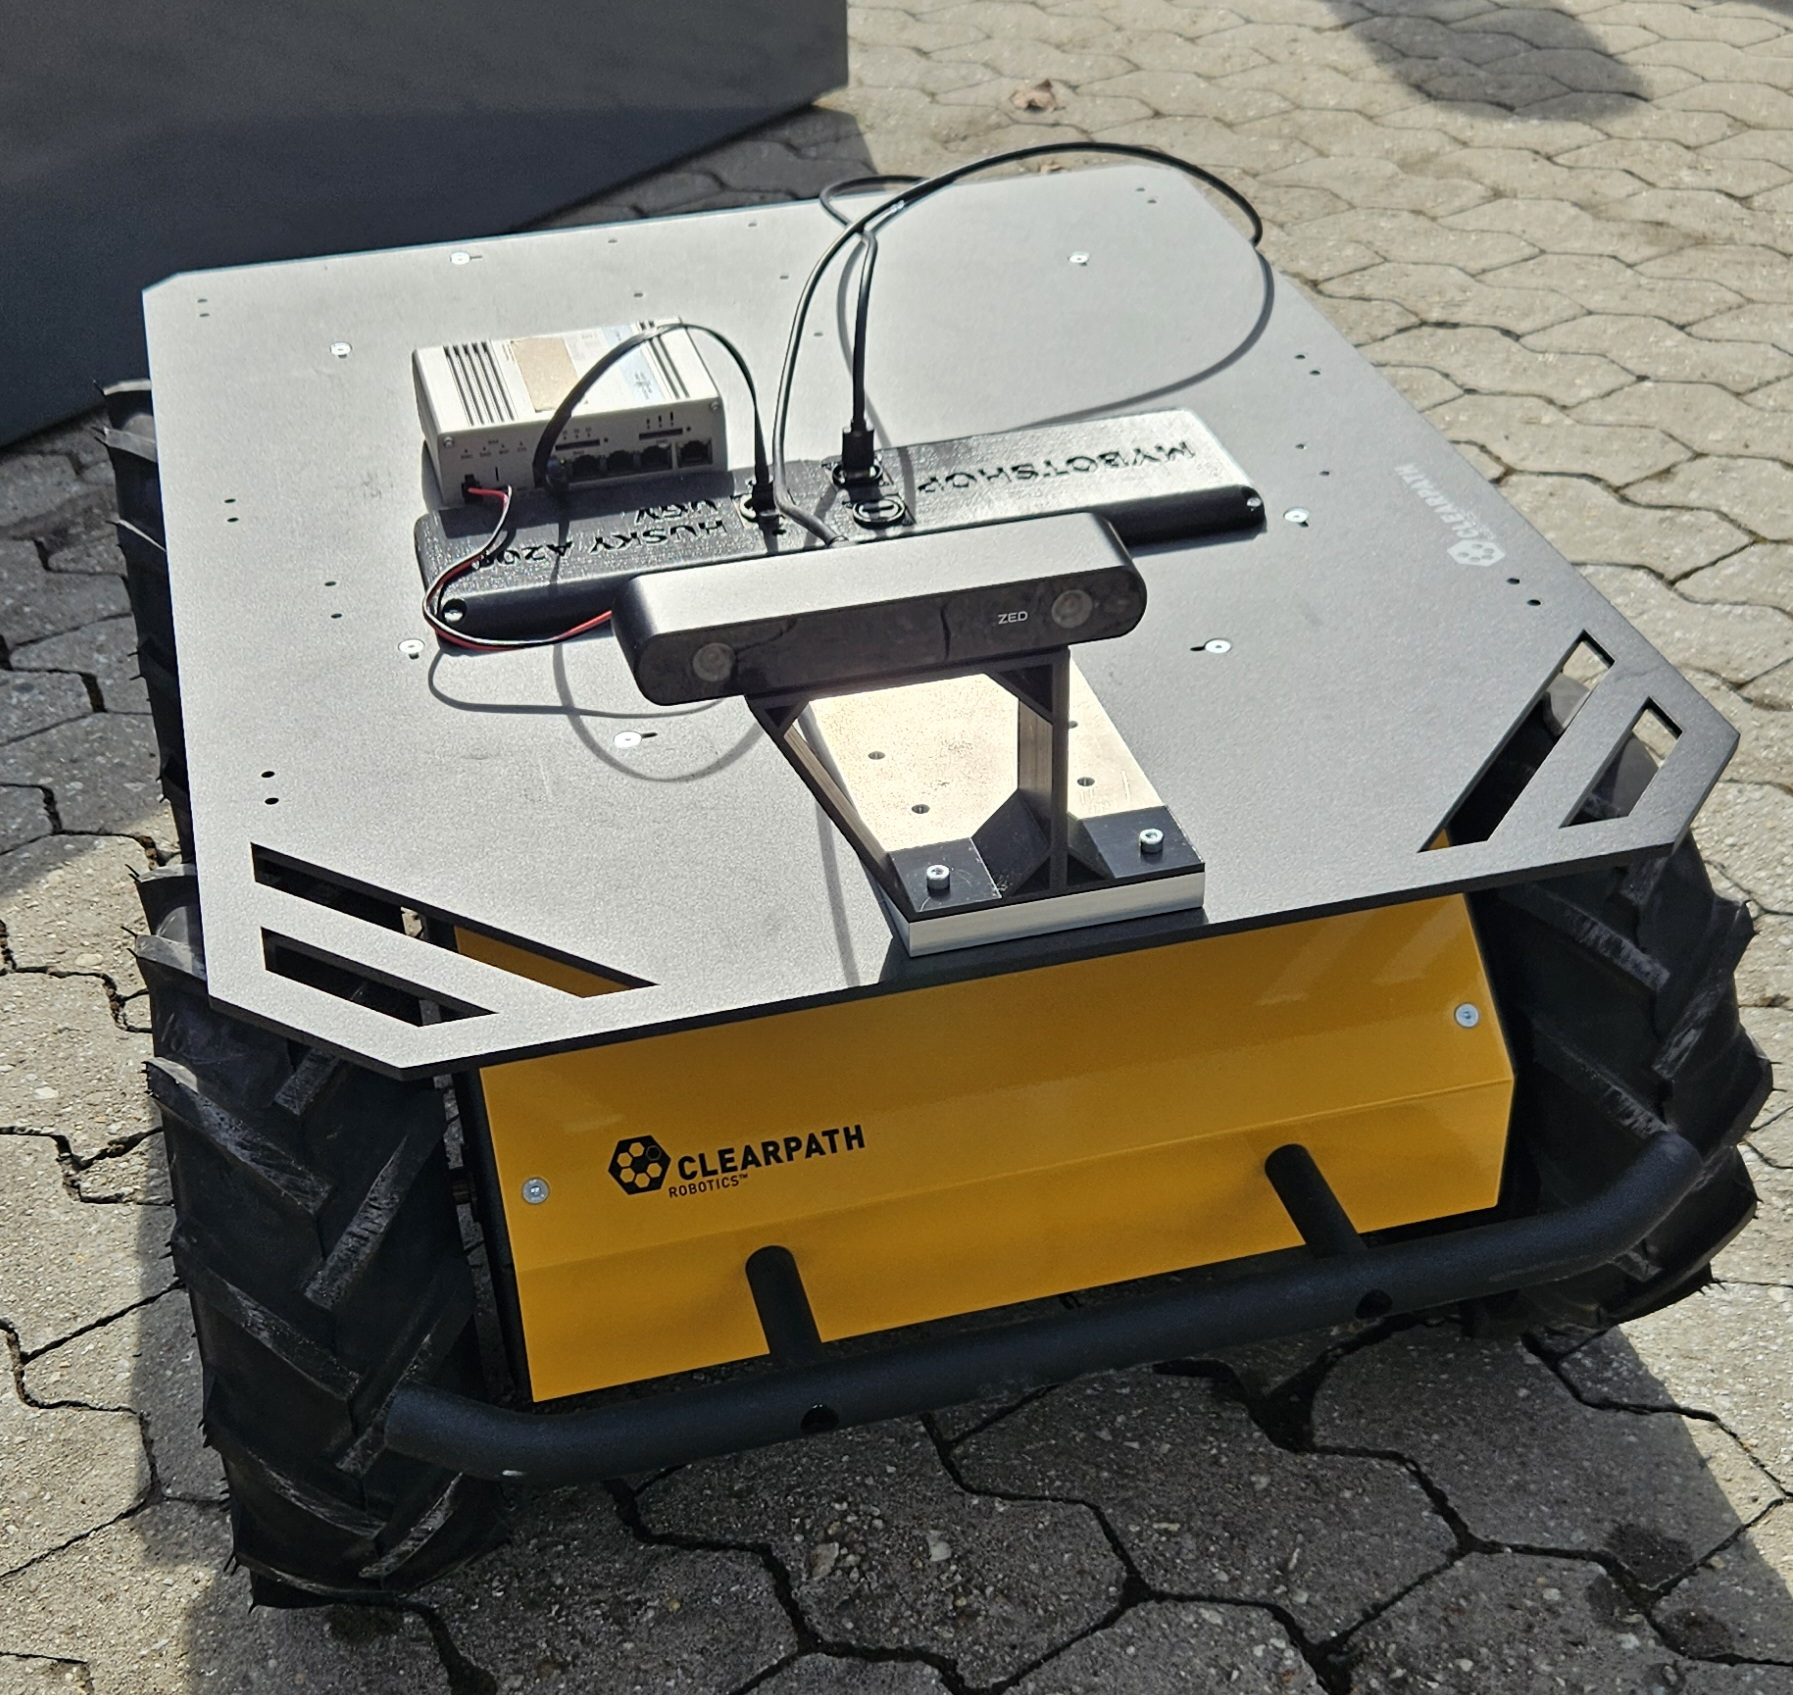
\includegraphics[width=8.cm]{Pictures/huskyzed2.jpg}}
	\caption{The Husky UGV by Clearpath Robotics as mobile robot with an attached Zed 2i stereo camera.}
	\label{fig:huskyClearpath}
\end{figure} 

The fusion of data  about the internal dynamic state collected by proprioceptive sensors, such as  odometry sensors, and external environment state captured by exteroceptive sensors, such as the camera in \cref{fig:huskyClearpath}, has  recently been pointed out to improve the performance of robotized systems of systems (SoS) in terms of perception and shared control \cite{chen2023enabling,kaigom}. We argue that endowing DTs with such a multi-modal and complementary  data-driven capture of visual (i.e., external) and behavioral (i.e., internal)  properties of SoS in real-time elevates situational awareness and facilitate informed decision making in applications  propelled by DTs. %This is done while remotely, \textit{internally}, and \textit{spatially} not only monitoring but also steering a robot to reach a desired location. 

\begin{figure*}[t]
	\centerline{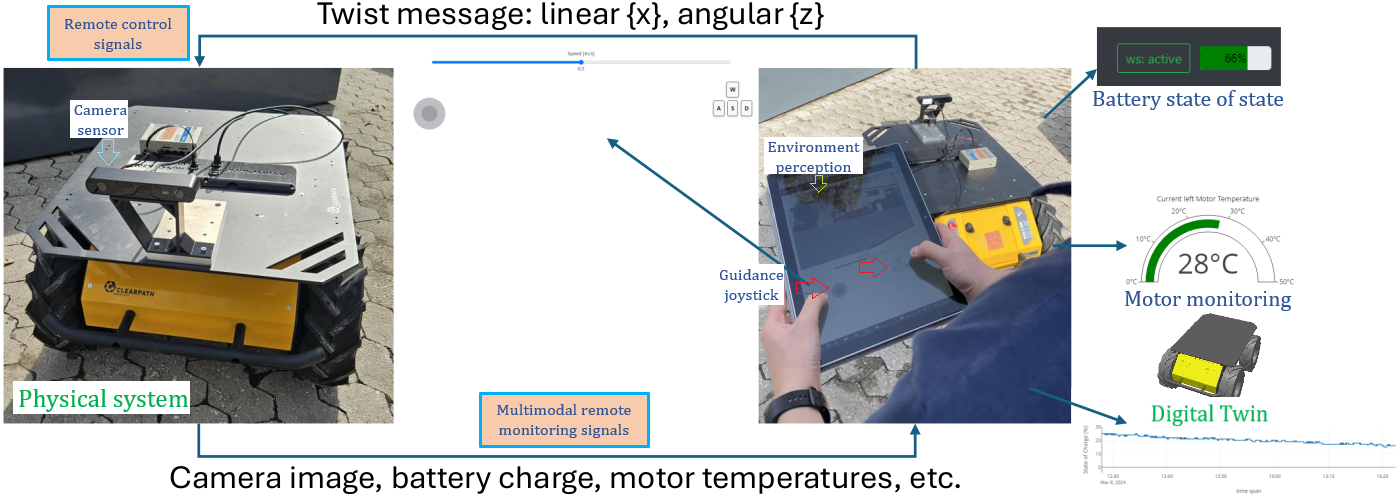
\includegraphics[width=16.35cm]{Pictures/loop.png}}
	\caption{Data loop between the Husky UGV robot and the web user interface}
	\label{fig:loop}
\end{figure*}
 
\section{Contribution}
In response to this need, we describe the development of a platform-independent and location-agnostic web application for the visual-proprioceptive supervision and active guidance of mobile robots
using their multimodal DTs. 
Users gain access to critical live information, including immediate environment constraints, obstacles, battery status, and motor temperatures, which are all provided on the intuitive web interface. This ensures widespread accessibility usability from everywhere. Conversely, even novices  harness the interface to guide the robot in real-time while remaining aware of its internal dynamics and external perception. This helps combine human cognitive skills with machine intelligence, facilitates the anticipation \mbox{of constraints and accommodation of uncertainties.}

%We describe the development and employment of  multimodal DTs (mDTs) for the vision-proprioceptive supervision and active guidance of mobile robots. Our approach is open, platform-agnostic, and accessible from everywhere my means of web-functionalities. It is suitable even to novices and supports industrial \mbox{communication standards, such as OPC UA.} 


%The Robot Operating System (ROS) stands as a ubiquitous middleware framework in the realm of robotics serving as a foundational platform for constructing robot systems and developing robot applications \cite{rosOrg}. 
%However, for individuals possessing limited or no prior exposure to robot software, navigating the intricacies of ROS can prove challenging. 
%This challenge is particularly pronounced for users who rely on robotic assistance and require an intuitive means of interacting with these machines.



%In response to this need, we have developed a platform-independent web application. 
%Designed with accessibility in mind, this application facilitates seamless monitoring and control of a locally networked robot. Users gain access to critical information, including battery status and motor temperatures which are all presented through an intuitive web interface. 

%Notably, this application is compatible with any device supporting web browsers, ensuring widespread accessibility and usability.

\begin{comment}
The robotic platform employed in our research is the Husky Unmanned Ground Vehicle (UGV) manufactured by Clearpath Robotics. This medium-sized mobile robot depicted in  \cref{fig:huskyClearpath,fig:loop} operates on  ROS2 distribution Humble Hawksbill.
The Husky UGV provides a maximum payload capacity of 75 kg and is therefore suitable for transporting and accommodating various auxiliary components to form rSoS. Researchers can mount additional robots, peripherals and specialized tools on this versatile platform. Its robust design and adaptability make it an ideal choice for a wide range of robotic applications. \cite{huskyClearpath} 
\end{comment}


\section{State of the Art}
In \cite{kapic} a Python web application was developed with the Django framework that uses a single virtual joystick with the objective to teleoperate the TurtleSim robot within a simulation environment. 
Therefore, a WebSocket connection and the ROS (Robot Operating System) \cite{rosbridgeOkState} JavaScript library Roslibjs were used to send commands from the web application to the robot. Specifically, the web application dispatched a twist message composed of vector components representing both linear and angular motion to the robot. This message effectively guided the robot's movements, enabling teleoperation.
The Rosbridge protocol constitutes a pivotal component within the ROS ecosystem. As a ROS package (rosbridge\_suite), it includes a WebSocket server and uses the Roslibjs library. Its primary purpose lies in establishing a robust foundation for communication, leveraging the JavaScript Object Notation (JSON).
Specifically, the Rosbridge protocol enables programming languages capable in handling JSON to communicate with ROS via the Rosbridge. 
This enables external systems and applications to perform various operations, such as subscribing to or \mbox{publishing ROS topics while avoiding active polling. \cite{rosbridgeOkState,rosbridgeSuite}}

In \cite{dinodi} a web application was developed with the primary objective of moving a Turtlebot3 in a virtual simulation environment with image transmission and autonomous navigation options. A virtual joystick was also made available to the user for manual control. Similarly to the first application, the communication between the app and the Turtlebot3 is facilitated with Rosbridge. 
One of the core aspects of the app is to bring robots closer to beginners and those interested in ROS. 
The app makes use of a range of frameworks and ROS-specific software. Among others, ReactJS, a JavaScript library was used for the frontend and to create the virtual joystick. For the backend, NodeJS and ExpressJS frameworks were used to open the ROS simulation environments. 
The authors state that only minimal knowledge of robotics is required to use the application. The app is freely accessible  through web access.

In \cite{johnson} a web platform was developed that deals with social robot application development. A physical Baxter robot and a virtual Baxter robot in the Gazebo ROS simulation environment were used. In essence, it is about web-based interpretation of social signals, hybrid block/text scripting interfaces and ROS integration via Rosbridge. 
The web components were created using JavaScript. The Baxter robot is equipped with a camera whose video stream is accessible to users via the ROS package web\_video\_server \cite{webvideoserver}.\\
A live remote interaction platform called TeleRobot was developed in \cite{wang}. This is also based on Rosbridge to interact with serveral robots and WebRTC to transmit images and audio in real-time. The main focus of this platform is to make robots accessible to users. The robots are controlled via a control panel. Other features include live chat, live streams, user management and an integrated database.

\section{Implementation and Design}
The system architecture of our web application is made up of backend and frontend components. These components synergistically leverage an array of tools and frameworks to facilitate seamless monitoring and guidance of mobile robots using their DTs. \Cref{fig:loop} shows the general idea of the data loop between the Husky UGV robot \cite{huskyClearpath} and  web application.

\subsection{Backend}
Our web application is built using Flask, a micro web framework designed for Python.
Flask offers core features and extensions to swiftly develop web applications. Flask is also very flexible and highly expandable \cite{flasksqlite}. The following tools are used in the backend:

\begin{itemize}
\item SQLAlchemy is a Python SQL toolkit and can be integrated into Flask as an extension. SQLAlchemy allows users to link Python objects to SQL databases using Object-Relational Mapping (ORM). This allows, for example, database queries to be made using Python code instead of SQL commands. The extension is also database-agnostic. 
Python code can be used unchanged for various SQL-based databases such as SQLite, PostgreSQL or MySQL. \cite{sqlalchemy} 
SQLite is used as a database to store ROS and user data pertaining to the DT. It is a serverless database, and directly performs read and write operations on standard disk files. This characteristic renders it operable in a self-contained manner, devoid of any supplementary software dependencies or additional configuration settings. Consequently, it exhibits resource efficiency by minimizing the utilization of computational resources \cite{sqlite}, from which DT-based  applications in-motion and underlying services benefit. 
\item The Roslibjs JavaScript library and the Rosbridge v2.0 protocol are used to establish bidirectional communication with the robots and the web application. The Rosbridge server which it contains, provides a WebSocket connection so that web browsers can communicate with Rosbridge.
Roslibjs is employed as a JavaScript library to interact with ROS topics, enabling the subscription to and publication of these topics. \cite{rosbridgeOkState, rosbridgeSuite} Hence,  the DT can mediate as monitoring interface without active polling.

Conversely, a prominent control and guidance application of this interaction is the publication of a geometry\_msgs/Twist message on the /cmd\_vel topic of the Husky robot which initiates its movement.
The geometry\_msgs/Twist message is composed of linear and angular vectors, which represent the velocity in free space \cite{twistmsg}. Specifically, these vectors are expressed in terms of meter per second and radian per second, respectively, in a right-handed coordinate system.
In the context of the Husky robot, a linear velocity of 1 meter per second in the positive x-direction corresponds to forward movement at a speed of 1 meter per second. To induce rotational movement, an angular velocity is specified in the z-direction \cite{huskydriving}. Positive and negative values correspond to counterclockwise and clockwise rotations respectively.
\item Keyboardteleopjs facilitates the translation of physical keystrokes into robot movements (see r.h.s of \cref{fig:loop}). A message is sent to the /cmd\_vel topic by pressing a key on the keyboard to set the robot in motion. \cite{keyboardteleopjs}
\item The Web Video Server is a ROS package that allows HTTP streaming of ROS image topics \cite{webvideoserver}. This integrates the live image from a Zed 2i camera from StereoLabs \cite{zed} into the web interface (see r.h.s of \cref{fig:loop}).

\item Flask-Login and Werkzeug.security extensions are used to handle login, logout, and session functions as well as to enhance user password security through password hashing \cite{flasklogin, werkzeug}. Additionally, it is possible to register new user accounts and assign permissions to different user roles to further preserve privacy along with scalability. 
\end{itemize}

\Cref{fig:userapp} illustrates the backend architecture and the method by which users can interface with the Husky robot via the web application while being informed by its DT. This system is designed to operate on \textit{any} device equipped with a web browser, utilizing the IP address of the Husky's onboard computer for connectivity.
The user interface provides real-time access to a live stream from a Zed 2i camera as well as control options for the robot. Additionally, it displays current ROS data, including metrics such as the battery State of Charge (SoC) and motor temperatures (see also r.h.s of \cref{fig:loop}).

A key feature of the developed system is its ability to track and store historical and live data in (not only) the SQLite3 database. The mobile robot turns out to be a mobile data hub. Data stored in it can be transformed into competitive advantages by harnessing edge AI. Doing so adheres to the vision pursued by our overarching value-driven DTs \cite{kaigom2020value} and Metarobotics \cite{kaigom} frameworks to create a global, digital, and parallel  intelligence for robot-driven industrial and societal applications. As depicted in \cref{fig:3dreal}, we strive is to deploy e.g. collective, foundational, generative, and transferable Artificial Intelligence/Machine Learning techniques to support the pervasive and itinerant access to services for the completion of remote robotized applications. These include design, development, automation, maintenance, safety, and sustainability as a service. Next generation wireless communication and immersion, as well as decentralized and interoperating DTs of existing and prospective assets are leveraged to this end. Such DTs are assumed to even learn from each others to accelerate the creation of non-nominal values by taking advantage of particularities, singularities, and differences \cite{kaigom}. In particular, a longitudinal analysis of the robot's business and operational data can be instrumental in creating values. These include an improved robot design and usability for citizen satisfaction (Society 5.0),  smart and efficient production and maintenance (Industry 4.0), \mbox{as well as worker well-being (Industry 5.0).} %Related DT might then learn from each other tu push back current frontiers and 
%This system provides a flexible and accessible platform for robot control and data monitoring. 
%This underscores the potential of web-based interfaces in enhancing the usability and functionality of robotic systems. 
%The use of an IP-based connection protocol further emphasizes the system's adaptability and broad accessibility. The incorporation of a database for data tracking and storage demonstrates a commitment to data-driven decision making and performance optimization. 
\begin{figure}[t]
    \centerline{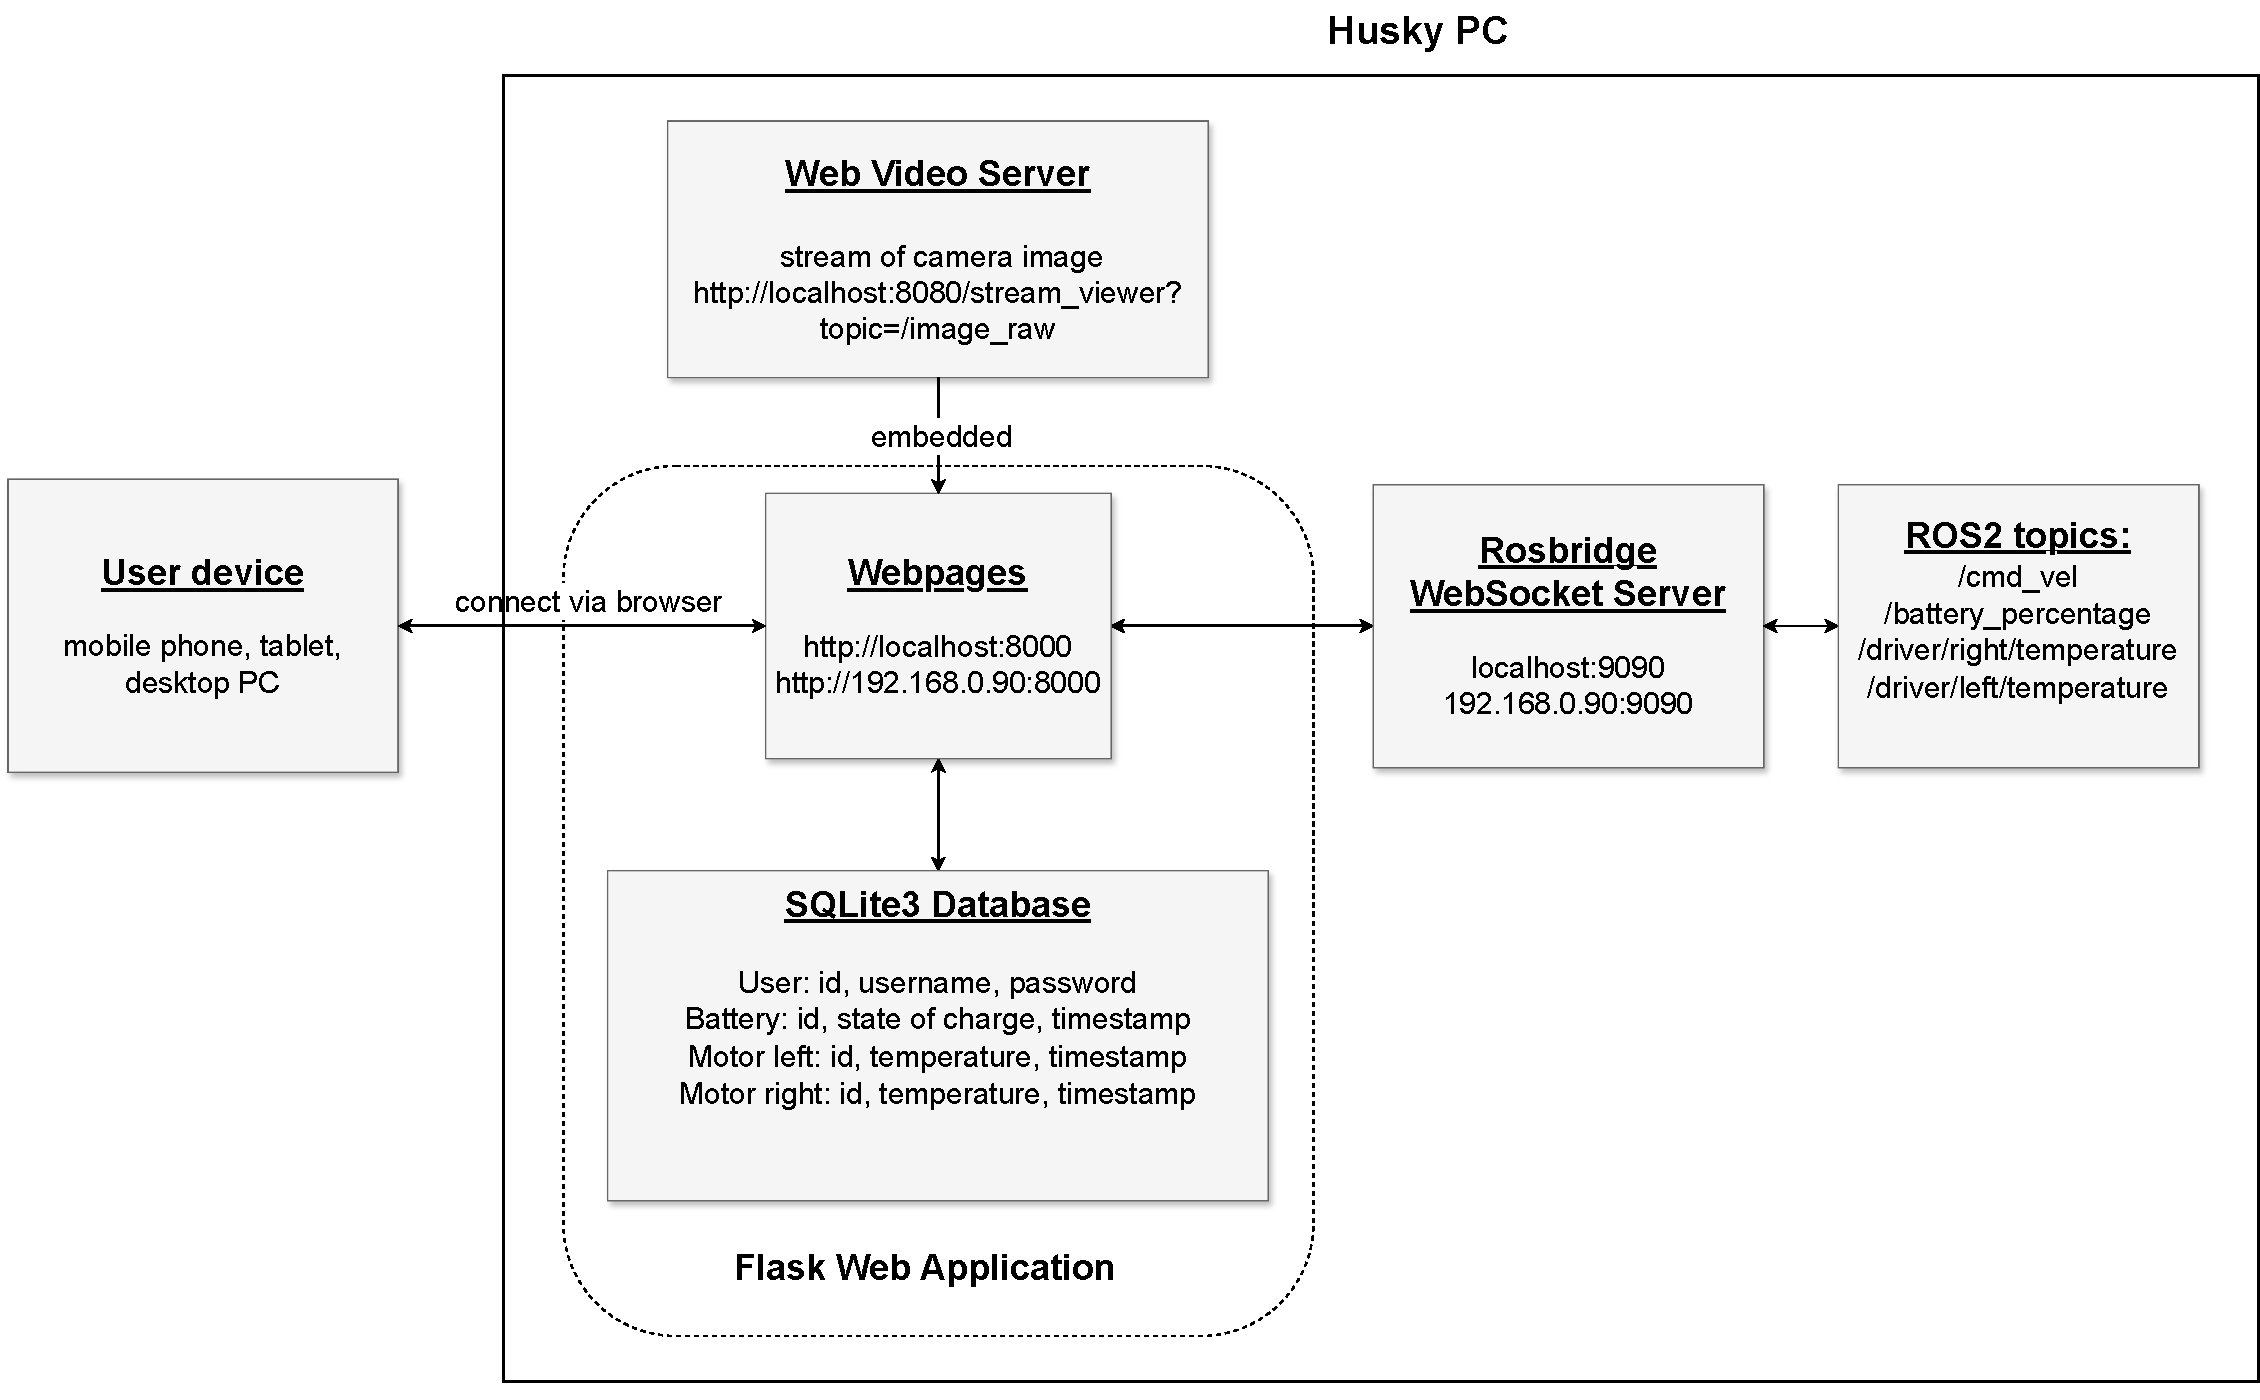
\includegraphics[width=8.9cm]{Pictures/userappbig.pdf}}
    \caption{Backend architecture of the web app}
    \label{fig:userapp}
\end{figure}
\subsection{Frontend}
An objective of the frontend design is to enhance user-friendliness through visually intuitive components. Furthermore, the application aims for platform independence, ensuring that users are not constrained by specific devices when accessing the web user interface. 
To achieve this, the web application is developed to be compatible with a wide range of devices including desktop PCs and mobile devices (see \cref{fig:galaxysurface}). Implementation details and outcomes of the individual frontend design tools presented here are shown in \ref{VS}.
\begin{itemize}
\item Leveraging on the free and open-source CSS framework Bootstrap version 4.6, we optimize responsiveness and integrate with prevailing web standards such as HTML5, CSS3, and JavaScript \cite{bootstrap}. 
In the context of Bootstrap, the layout structure is organized using the grid system for arranging elements and components within a web page. 
Additionally, a navigation bar is crafted to reinforce user navigation.
Furthermore, the implementation of a battery display is achieved through the utilization of the Bootstrap class .progress-bar. 
This class enables precise control over visual representations of battery levels or  progress indicators (see r.h.s of \cref{fig:loop}).
\item Plotly.js, an open-source graphing library serves as a tool for constructing interactive and touch-enabled visualizations. It facilitates the creation of dynamic plots that allow users to zoom in and out as well as capture screenshots of relevant data, \cite{plotly} (see r.h.s of \cref{fig:loop}). 
\item The Husky robot is equipped with a physical motion controller by default. Teleoperation is achieved through the utilization of an analog joystick and the left and right shoulder buttons to set a specific maximum velocity \cite{huskydriving}.
We streamline, extend and transfer this functionality to the web interface. Nipple.js is used to this end. This library enables the configuration and display of a virtual joystick \cite{nipplejs} (see \cref{fig:loop}). Also, a horizontally scrollable velocity slider is created using the Bootstrap class .form-control-range to set a desired maximum speed (see \cref{fig:loop}).
\item The app exhibits versatility in its control mechanisms. Users have the option to teleoperate the robot via a physical keyboard, provided they have one readily available. For users without  physical keyboard connection, an alternative method involves utilizing the custom “WASD” touch keys displayed within the application interface. 
These touch keys can also be used for the robot movement. The Husky can be driven more precisely using the keyboard buttons. This is useful when, e.g., parking.
\item Three.js is a powerful and lightweight 3D graphics library that can be served as a versatile tool for rendering digital representations of robots within web browsers \cite{threejs}. In future work a combination with Ros3djs can be considered to further implement and reflect in terms of animations the live movements of the real robot on the browser \cite{ros3djs}. For example, a blinking or lighting up of the visualized husky in the browser when the battery SoC is low. 
As an ongoing project, we have successfully integrated a 3D model  of the Husky as part of its DT into our application as a proof of concept (see r.h.s of \cref{fig:loop}).
\end{itemize}

\subsection{Interaction between backend and frontend}
The value of the battery SoC is used as an example to explain the data flow between the backend and frontend. 
\subsubsection{Direct display of the battery SoC}
The current value of the battery SoC which is published by the ROS topic /battery\_percentage is visualized directly in the user interface with Bootstrap each time the message is received. For this purpose, a ROSLIB.topic object is created beforehand in JavaScript that subscribes to the corresponding ROS topic, allowing real-time updates. It is also possible to send messages to this topic, as is the case with the Husky teleoperation. 
In this case the virtual joystick position sends a twist message to the /cmd\_vel topic to move it. 
The connection between the app and the Husky is established via the WebSocket. 
\subsubsection{Capturing the values}
In the backend, a route is defined in the Flask web application that listens for HTTP POST requests at the /save\_data endpoint. If a POST request is received, the incoming JSON data is queried. In this scenario, a battery object is then created with the percentage value. The object adds it with an id and a timestamp to the database session (Fig. \ref{fig:userapp}). In the event of a database failure, the current battery SoC can still be displayed. The same applies to the engine temperatures (see \cref{fig:backfront}).
\subsubsection{Visualizing the data from the database}
The SoC for the battery is visualized using Plotly.js as a line chart. This process involves several steps. Initially, data are fetched from the backend database. After processing to ensure compatibility with Plotly.js, it is prepared for visualization. The resulting line diagram represents the battery SoC over a certain time span. Flask facilitates the transfer of Python variables to the frontend. 
These variables are utilized within HTML templates or JavaScript via Jinja, a template engine \cite{jinja}. Users can interact with the system by selecting specific days from a drop-down list. \mbox{Recorded data related to the chosen day are displayed.}
\begin{figure}[tp]
    \centerline{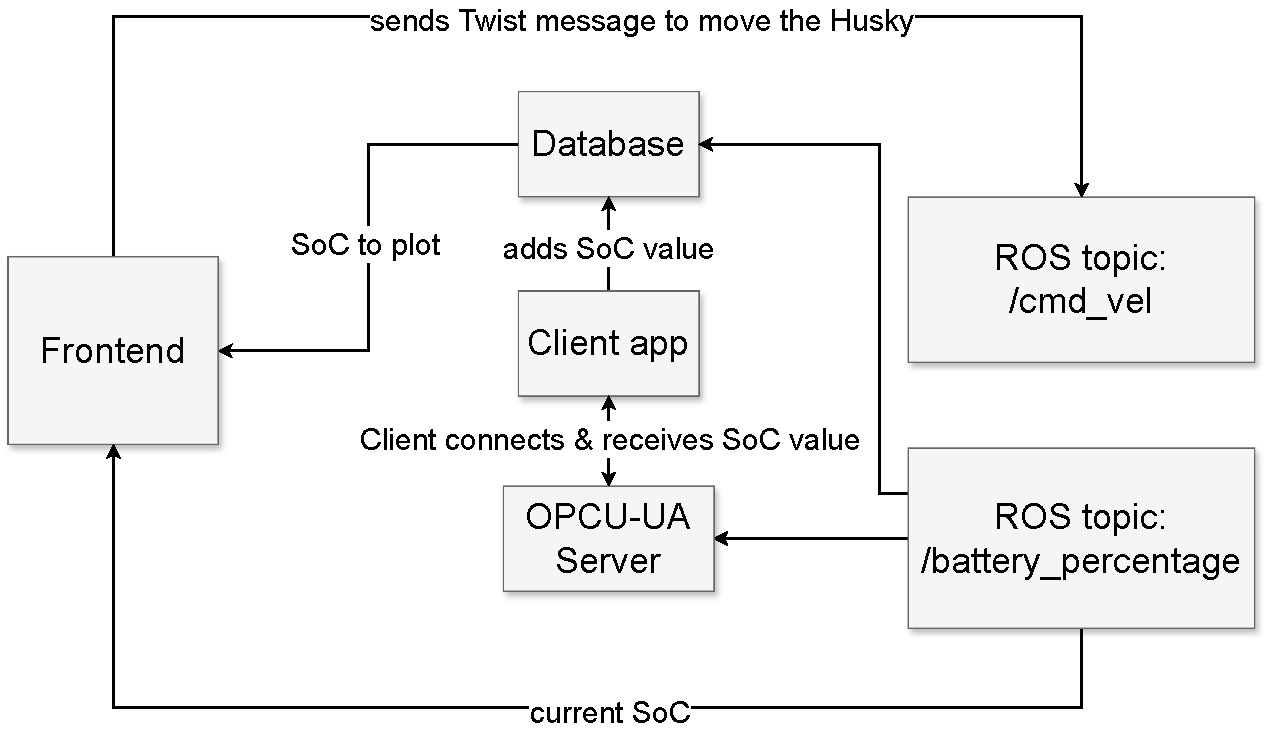
\includegraphics[width=8.9cm]{Pictures/backfrontbig.pdf}}
    \caption{Interaction between frontend and backend}
    \label{fig:backfront}
\end{figure}
\subsubsection{Connecting to an Open Platform Communications Unified Architecture Server}
A pre-existing DataConnector (DC) has been specifically developed for the Husky as part of a prior project. This DC leverages the Open Platform Communication Unified Architecture \cite{opcua} (OPC-UA) standard. Through this industry-compatible connector,  ROS data from the Husky are efficiently retrieved. The retrieval process is facilitated by a client program integrated into the web application and the acquired data are persistently stored in the database. 
In the event of an OPC-UA server failure, the system is designed to continue displaying the real-time ROS \mbox{data of the Husky (\cref{fig:backfront}).}


\section{Validation and Showcase}\label{VS}
To test the responsiveness of the front end of the web application, the app was accessed from different devices. The Flask application can run on the Husky's onboard PC or on another PC in the same local network as the Husky with access to the ROS topics. The application was mainly tested on the mobile onboard PC (i5-1135G7 CPU and 16 GB RAM) to serve the locally stored files to the client.
The representation of the data page is shown in \cref{fig:galaxysurface}. 
\begin{figure}[b]
    \centerline{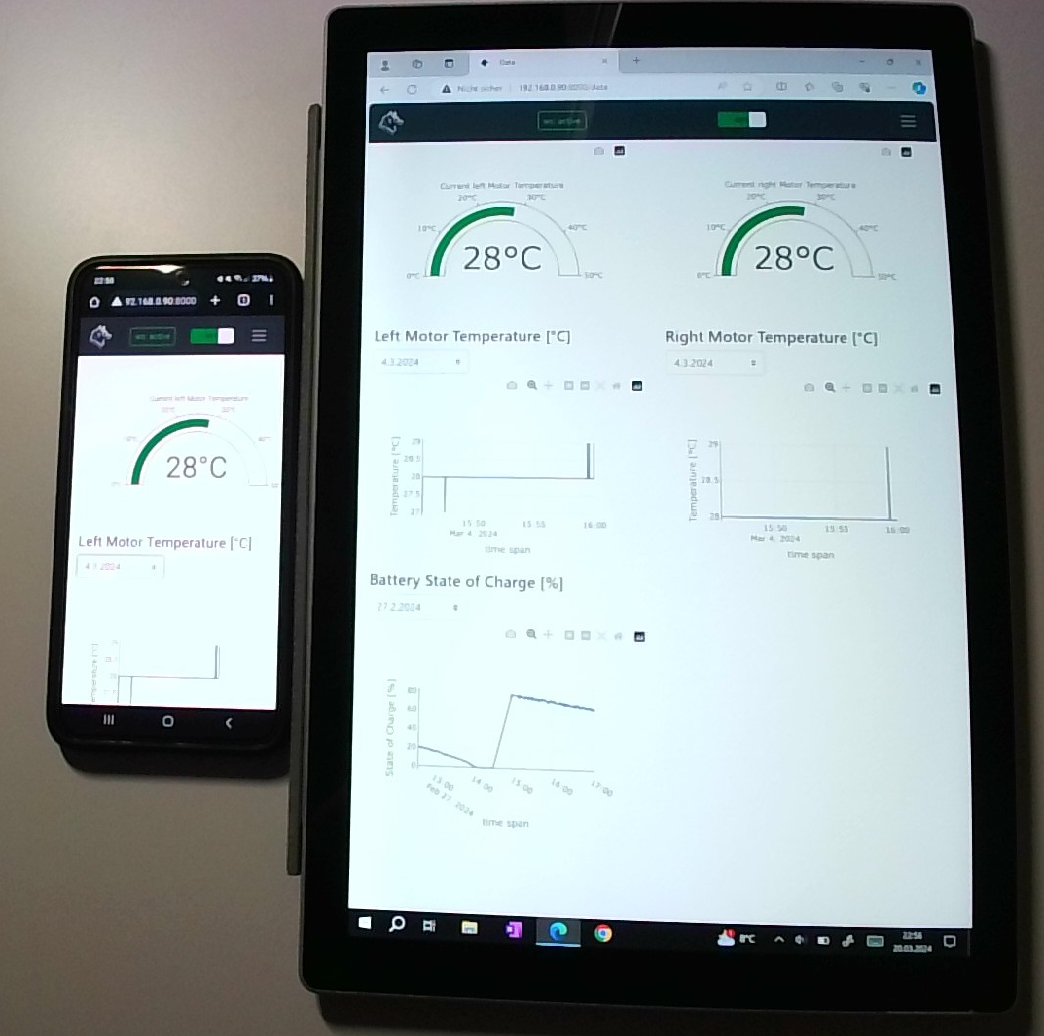
\includegraphics[width=6.cm, height=5.cm]{Pictures/galaxysurfacecut.png}}
    \caption{Galaxy S23  (l.h.s) and Surface Pro (5th Gen.) support the framework.}
    \label{fig:galaxysurface}
\end{figure}
In this experiment we investigate the visual representation of the web application interface across two distinct devices: a Samsung Galaxy S23 cell phone and a Microsoft Surface Pro tablet (5th Generation). The purpose is to discern how design elements and user experience differ between these platforms.
On the left hand side the data page was accessed using a Samsung Galaxy S23 cell phone while on the right hand side the site was displayed on the Surface Pro tablet.
Embedded within the navigation bar is a real-time indicator of the battery SoC at the top right corner. This value is updated dynamically as the Husky operates.
Additionally, a status display reflects the active WebSocket connection (next to the SoC), providing essential feedback to the user.
These components were developed with the Bootstrap framework. The current motor temperatures are visualized using angular gauge charts. These succinct representations allow rapid assessment of temperature levels.
Below that, the motor temperature data are plotted as line charts. Both visualizations were generated using Plotlyjs.
Positioned at the bottom left corner, a similar display exists for the battery SoC which can be seen on the Surface Pro tablet. Due to space constraints of the Galaxy S23 screen only a truncated version of the data page is visible in \cref{fig:galaxysurface}. To view the remaining gauge and plots on the Galaxy S23, it is required to scroll down. The visualizations are listed below each other.  
On both devices, the navigation bar undergoes compression, resulting in a more compact layout.
A convenient drop-down menu arrangement (top right) allows users to access elements sequentially by scrolling vertically (see \cref{fig:3dreal}).
The control interface in \cref{fig:galaxycontrol} features a live image display of a Zed 2i camera, which serves as the primary view. Positioned centrally, this display provides real-time visual feedback. Beneath the image, the speed slider resides. It is adjustable from 0.1 meter per second to a maximum of 1 meter per second and is accompanied by a numerical readout.
The interface includes touch-enabled controls: a virtual joystick positioned at the bottom left and virtual keyboard keys at the bottom right. These intuitive input mechanisms facilitate precise guidance control of the Husky robot. 
Their placement at the screen's edge aligns with the ergonomic orientation of handheld devices such as cell phones or tablets, enhancing user comfort and efficiency. 
\begin{figure}[b]
    \centerline{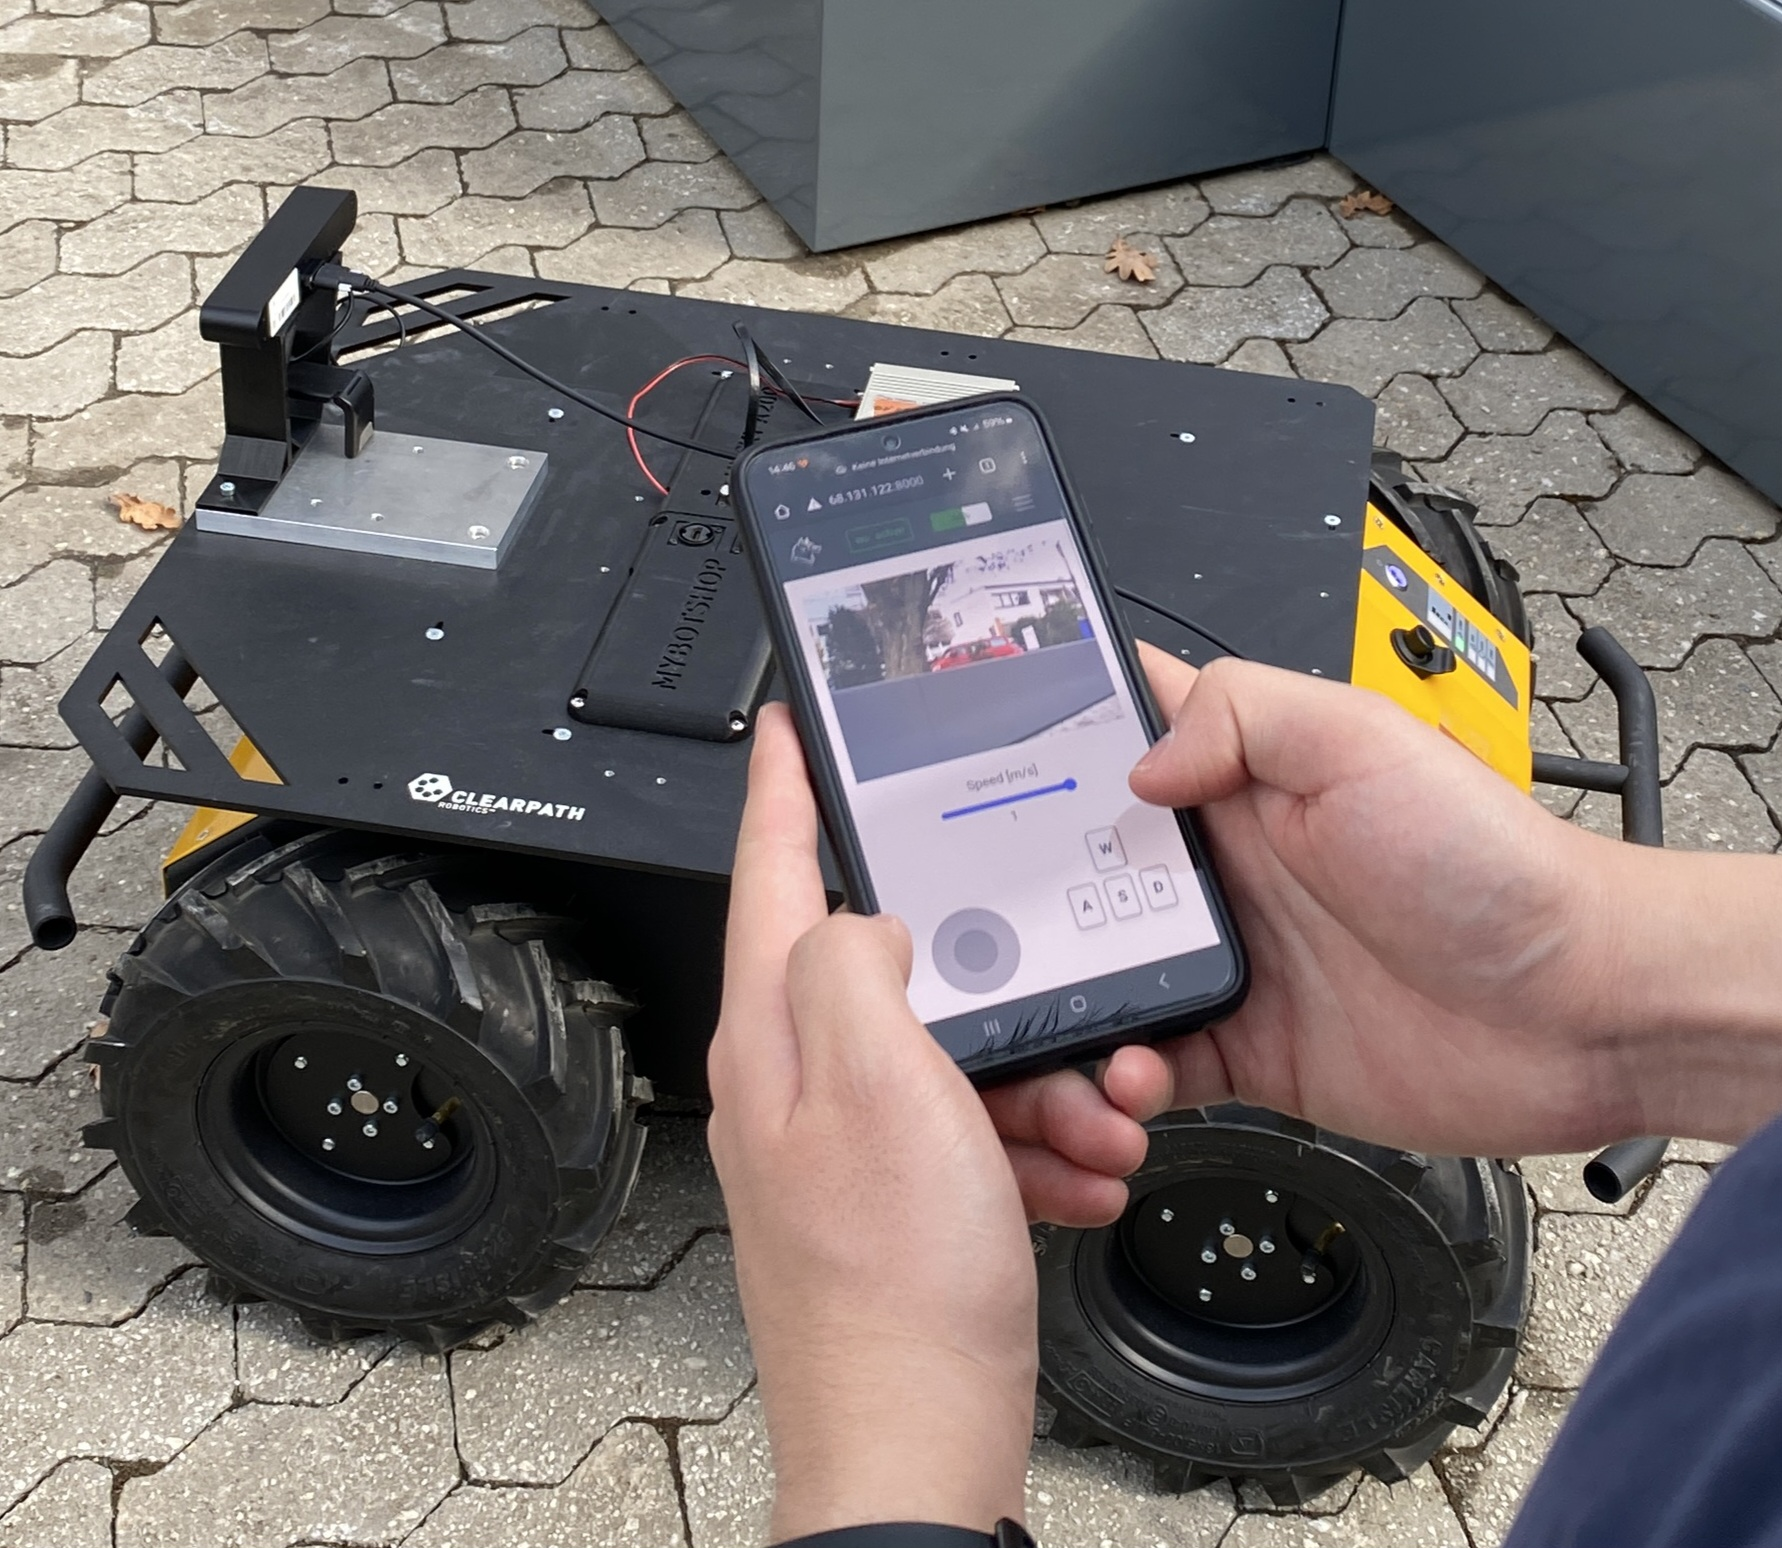
\includegraphics[width=5.3cm]{Pictures/galaxycontrol.jpg}}
    \caption{Control panel (mobile view with Galaxy S23) with battery soc, WebSocket status, live camera stream, virtual Joystick, speed slider, etc.}
    \label{fig:galaxycontrol}
\end{figure}
The 3D model route shows the visualized Husky as depicted in \cref{fig:3dreal}. It is possible to view the model from different angles.
The components listed here have been tested with the most common browsers such as Chrome, Firefox or Edge in different versions and on different devices. A list of supported browser versions of the Bootstrap components is available on the Bootstrap website \cite{bsBrowsers}. 
\begin{figure}[htbp]
    \centerline{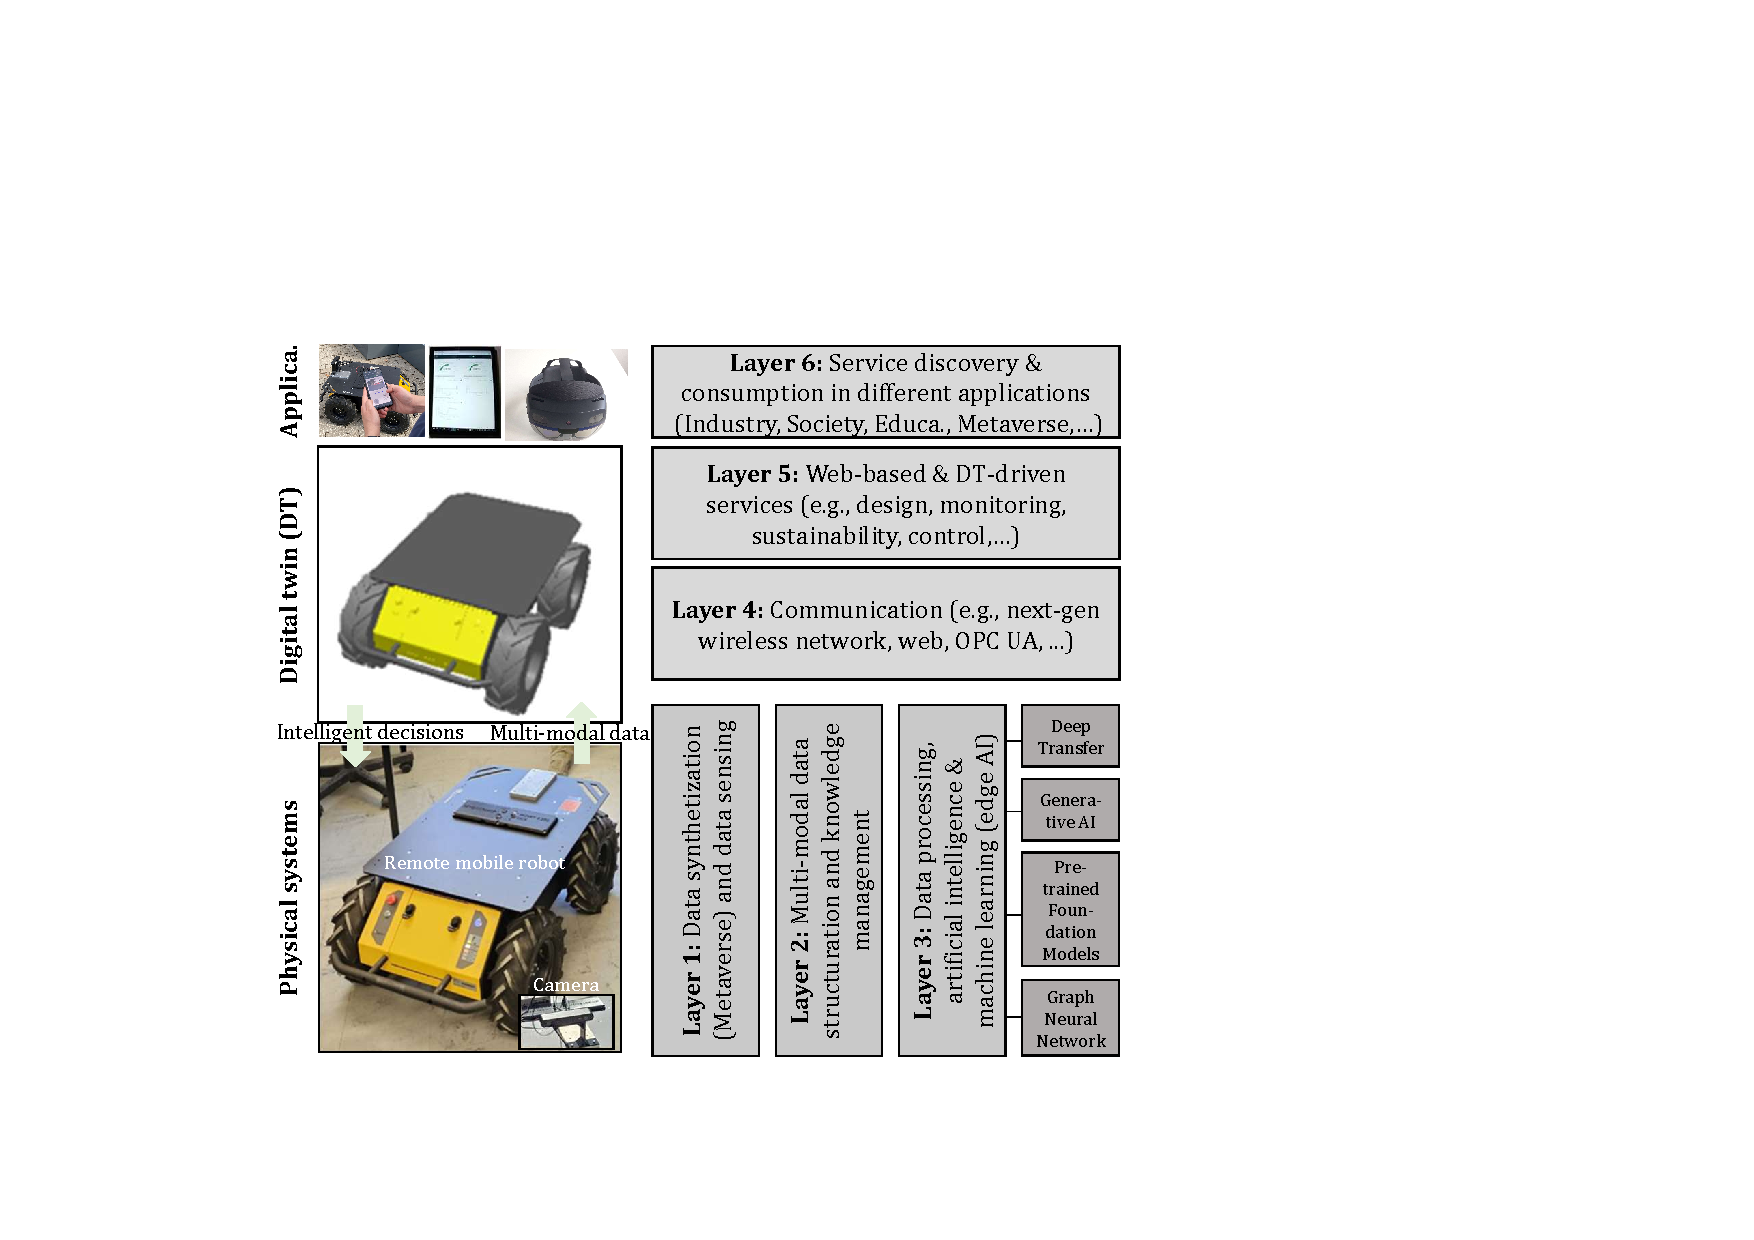
\includegraphics[width=0.98\columnwidth]{Pictures/layer0.pdf}}
    \caption{Basic overarching idea following \cite{kaigom,kaigom2020value}.}
    \label{fig:3dreal}
\end{figure}

\section{Discussion}
Our project synergistically integrates a constellation of frameworks and tools to achieve optimal functionality. In contrast to the comprehensive Python web framework Django, which provides an extensive feature set \cite{django} and was employed in \cite{kapic}, we have opted for Flask - a minimalist web framework that offers only fundamental functionalities. 
This choice allows us to selectively incorporate essential features and extensions, ensuring a streamlined and efficient self-hosted web application. 
Analogous to the context in \cite{kapic} and \cite{dinodi}, our application incorporates a virtual joystick.
The Husky's velocity can be modulated via a speed slider. Alternatively, teleoperation of the robot is achievable through keyboard input. Even in scenarios where a physical keyboard is absent, the mobile platform remains maneuverable using virtual keys. Particularly, the tactile keyboard keys afford finer-grained control compared to the virtual and physical joystick. 
Furthermore, consideration was given to the ergonomic arrangement of these components within the application, aligning with the natural posture observed during mobile device usage as shown in  \cref{fig:galaxycontrol}.
As in \cite{kapic}, \cite{dinodi}, \cite{johnson} and \cite{wang}, the robot data are transmitted to the app via the Rosbridge protocol and vice versa, which constitutes bidirectional communication. Similar to \cite{johnson}, a live camera feed was also integrated leveraging the Web Video Server.
Our backend system architecture also allows us to connect a specially developed OPC-UA server and client to write the Husky's ROS data to the database. In the event of database or OPC-UA server failure, critical ROS data such as the battery SoC or the engine temperatures remain accessible for real-time display (\cref{fig:backfront}).
The visual representation of the components within the web interface is also intuitive and has been built using the responsive Bootstrap frontend toolkit. This enables users to connect to the app as independently as possible from the respective web-enabled device with a customized display.

\section{Conclusion}
In this work, a web-based framework that facilitates the monitoring and control of the Husky robot has been developed. A multimodal digital twin approach is involved to reflect the internal dynamics and environmental context, as well as enabling a versatile control over the motion behavior of the remote mobile robot. 
Our framework supports devices with web connectivity, irrespective of their origin, or browser specifications. The framework integrates a robust database, enabling users to monitor and make  informed decisions from holistic real-time data over the robot. 
Additionally, visual representations enhance the presentation and interpretation of critical parameters, \mbox{such as motor temperature and battery status.}


\begin{thebibliography}{00}
%	\bibitem{li2023classification}Li, G., Li, Q., Yang, C., Su, Y., Yuan, Z. \& Wu, X. The classification and new trends of shared control strategies in telerobotic systems: A survey. {\em IEEE Transactions On Haptics}. (2023)
%\bibitem{wang2024bibliometric}Wang, J., Li, X., Wang, P. \& Liu, Q. Bibliometric analysis of digital twin literature: A review of influencing factors and conceptual structure. {\em Technology Analysis \& Strategic Management}. \textbf{36}, 166-180 (2024)
\bibitem{DT}"The global digital twin market size ," Fortune Business Insights, \url{https://www.fortunebusinessinsights.com/digital-twin-market-106246} (accessed March 23, 2024).
\bibitem{yang2023design}Yang, H., Cheng, F., Li, H. \& Zuo, Z. Design and Control of Digital Twin Systems based on a Unit Level Wheeled Mobile Robot. {\em IEEE Transactions On Vehicular Technology}. (2023)
\bibitem{chen2023enabling}Chen, Y. Enabling mobile robot perception and shared-control with vision-based sensor fusion systems. (PhD, University of Illinois at Urbana-Champaign,2023)
%\bibitem{rosOrg}"ROS - Robot Operating System," ROS, \url{https://ros.org} (accessed March 18, 2024).

\bibitem{kaigom}
Guiffo Kaigom, E.  "Metarobotics for Industry and Society: Vision, Technologies, and Opportunities". IEEE Transactions on Industrial Informatics, 2023.




\bibitem{kapic} Zinaid Kapić, Aladin Crnkić, Edin Mujčić and Jasna Hamzabegović, "A web application for remote control of ROS robot based on WebSocket protocol and Django development environment", in IOP Conf. Ser.: Mater. Sci. Eng. 1208 012035, 2021, doi: 10.1088/1757-899X/1208/1/012035.
\bibitem{rosbridgeOkState} Crick, C., Jay, G., Osentoski, S., Pitzer, B., and Jenkins, O. C. "Rosbridge: Ros for non-ros users" in Robotics Research, Springer, 2017.
\bibitem{rosbridgeSuite}"rosbridge\_suite," rosbridge suite - ROS Wiki, \url{http://wiki.ros.org/rosbridge\_suite} (accessed March 14, 2024).
\bibitem{dinodi} D. D. Rajapaksha et al., "Web Based User-Friendly Graphical Interface to Control Robots with ROS Environment," 2021 6th International Conference on Information Technology Research (ICITR), Moratuwa, Sri Lanka, 2021, pp. 1-6, doi: 10.1109/ICITR54349.2021.9657337.
\bibitem{johnson}Brisaac Johnson et al., "Towards Web-based Environments for Prototyping Social Robot Applications," in Companion of the 2021 ACM/IEEE International Conference on Human-Robot Interaction (HRI '21 Companion). Association for Computing Machinery, New York, NY, USA, 308-312, \url{https://doi.org/10.1145/3434074.3447182}.
\bibitem{webvideoserver}"web\_video\_server," ROS, \url{http://wiki.ros.org/web\_video\_server} (accessed March 20, 2024).
\bibitem{wang}X. Wang et al., "TeleRobot: Design and Implementation of a Live Remote Interaction Platform for Robots*," 2023 IEEE International Conference on Systems, Man, and Cybernetics (SMC), Honolulu, Oahu, HI, USA, 2023, pp. 408-412, doi: 10.1109/SMC53992.2023.10394406.
\bibitem{huskyClearpath}"Husky UGV - Outdoor Field Research Robot by Clearpath," Clearpathrobotics, \url{https://clearpathrobotics.com/husky-unmanned-ground-vehicle-robot/} (accessed March 17, 2024).
\bibitem{flasksqlite} Suraya, Muhammad Sholeh, "Designing and Implementing a Database for Thesis Data," in International Journal of Engineering, Science \& InformationTechnology (IJESTY) Volume 2, No. 1, 2022
\bibitem{sqlalchemy}"The Python SQL Toolkit and Object Relational Mapper," SQLAlchemy, \url{https://www.sqlalchemy.org/} (accessed March 20, 2024).
\bibitem{sqlite}"About SQLite," SQLite, \url{https://www.sqlite.org/about.html} (accessed March 20, 2024).
\bibitem{twistmsg}"geometry\_msgs/Twist Message," ROS docs, \url{https://docs.ros.org/en/diamondback/api/geometry\_msgs/html/msg/\\Twist.html} (accessed March 19, 2024).
\bibitem{huskydriving}"Driving a Robot," Clearpath Robotics docs, \url{https://docs.clearpathrobotics.com/docs/ros/tutorials/driving} (accessed March 19, 2024).
\bibitem{keyboardteleopjs}"keyboardteleopjs," keyboardteleopjs - ROS Wiki, \url{http://wiki.ros.org/keyboardteleopjs} (accessed March 22, 2024).
\bibitem{zed}"ZED 2," StereoLabs*, \url{https://www.stereolabs.com/products/zed-2} (accessed March 22, 2024).
\bibitem{flasklogin}"Flask-Login," flask-login readthedocs, \url{https://flask-login.readthedocs.io/en/latest/} (accessed March 20, 2024).
\bibitem{werkzeug}"Utilities," Werkzeug, \url{https://werkzeug.palletsprojects.com/en/\\2.3.x/utils/\#module-werkzeug.security} (accessed March 20, 2024).
\bibitem{kaigom2020value}Guiffo Kaigom, E. \& Roßmann, J. Value-driven robotic digital twins in cyber–physical applications. {\em IEEE Transactions On Industrial Informatics}. \textbf{17}, 3609-3619 (2020)
\bibitem{bootstrap}"Introduction," Bootstrap, \url{https://getbootstrap.co, m/docs/4.6/getting-started/introduction/} (accessed March 16, 2024).
\bibitem{plotly}"Plotly JavaScript Open Source Graphing Library," Plotly, \url{https://plotly.com/javascript/} (accessed March 21, 2024).
\bibitem{nipplejs}"nippleJS," NippleJS by yoannmoi, \url{https://yoannmoi.net/nipplejs/} (accessed March 21, 2024).
\bibitem{threejs}"Creating a scene," threejs docs, \url{https://threejs.org/docs/index.html\\\#manual/en/introduction/Creating-a-scene} (accessed March 21, 2024).
\bibitem{ros3djs}"3D Visualization Library for use with the ROS JavaScript Libraries," ros3djs - ROS Wiki, \url{http://wiki.ros.org/ros3djs} (accesssed March 21, 2024).
\bibitem{jinja}"Template Designer Documentation," Template Designer Documentation - Jinja Documentation, \url{https://jinja.palletsprojects.com/en/3.0.x/templates/} (accessed March 22, 2024).
\bibitem{opcua}"Unified Architecture," Unified Architecture - OPC Foundation, \url{https://opcfoundation.org/about/opc-technologies/opc-ua/} (accessed March 22, 2024).
\bibitem{bsBrowsers}"Browsers and devices," Getbootstrap, \url{https://getbootstrap.com/docs/4.6/getting-started/browsers-devices/} (accessed March 17, 2024).
\bibitem{django}"Django makes it easier to build better web apps more quickly and with less code.," The web framework for perfectionists with deadlines., \url{https://www.djangoproject.com/} (accessed March 22, 2024).
\end{thebibliography}
\vspace{12pt}


\end{document}
